\message{ !name(dissertation.tex)}{\makeatletter\gdef\AucTeX@cite#1[#2]#3{[#3#1#2]}\gdef\cite{\@ifnextchar[{\AucTeX@cite{, }}{\AucTeX@cite{}[]}}}

\message{ !name(dissertation.tex) !offset(-3) }
%%%%%%%%%%%%%%%%%%%%%%%%%%%%%% -*- Mode: Latex -*- %%%%%%%%%%%%%%%%%%%%%%%%%%%%
%% _region_.tex -- 
%% Author          : Carleton Moore
%% Created On      : Mon Oct  5 10:45:35 1998
%% Last Modified By: Carleton Moore
%% Last Modified On: Tue Sep  7 15:01:37 1999
%% RCS: $Id$
%%%%%%%%%%%%%%%%%%%%%%%%%%%%%%%%%%%%%%%%%%%%%%%%%%%%%%%%%%%%%%%%%%%%%%%%%%%%%%%
%%   Copyright (C) 1998 Carleton Moore
%%%%%%%%%%%%%%%%%%%%%%%%%%%%%%%%%%%%%%%%%%%%%%%%%%%%%%%%%%%%%%%%%%%%%%%%%%%%%%%
%% 

%% The options are (you can only choose one from each group):
%%
%% 10pt, 11pt, 12pt: chooses the point size for the document. "11pt" is the
%%                   default.
%%
%% oneside, twoside: whether you want your document onesided or twosided. Note
%%                   that twosided is not guaranteed to work, and style
%%                   guidelines prohibit double sided printouts on final
%%                   copy. "oneside" is the default.
%%
%% draft, final: when printing drafts you can save a lot of paper by using the
%%               "draft" option. It switches to single spacing, displays overful
%%               hboxes with a black box, prints a version number on title page 
%%               and omits signature page. Of course for the final copy make
%%               sure to use the "final" option! "final" is the default.
%%
%% cm, times, palatino, newcent, bookman: switches between different font
%%                                        sets. "cm" is the Computer Modern
%%                                        font (TeX's default), the rest are
%%                                        PostScript fonts. "times" is the
%%                                        default.
%%
%% thesis, dissertation: switches between the style for a master's thesis and a 
%%                       Ph.D. dissertation. The differences are fairly minor
%%                       and limited to the front matter. "thesis" is the
%%                       default.
%%
%% actual, proposal: switches between actual document and proposal mode. In
%%                   proposal mode: the title page is simplified, the
%%                   version number is always printed, and the signature page
%%                   is omitted.
%%
%%% Load the uhthesis2e document class
\documentclass[11pt,times,dissertation,proposal]{uhthesis2e}

%%% Load some useful packages:
%% New LaTeX2e graphics support
\usepackage{graphicx}
%% Package to linebreak URLs in a sane manner.
\usepackage{url}

%%% End of preamble
\begin{document}

%%% Declarations for Front Matter. Capitalize all of these values
%%% "normally". This allows the document class to format them properly.
%% Full title of thesis or dissertation, capitalized like a title should be.
\title{LEAP:  A Lightweight, Empirical, Anti-measurement dysfunction, 
  and Portable approach to software developer improvement}
%% Your name, capitalized normally. Do not include any titles like Dr.
\author{Carleton A. Moore}
%% Month in which you intend to receive your degree (i.e. graduation).
%% Presumably this will be one of: May, August, or December.
\degreemonth{May}
%% Year of expected graduation.
\degreeyear{2000}
%% Type of degree to be conferred.
\degree{Doctor of Philosophy}
%% This is the chairperson of your committee. Do not use titles like Dr.
\chair{Philip Johnson}
%% The other members of your committee, seperated by "\\". Again, no titles,
%% and it is customary to list the outside committee member (if you have one)
%% last.
\othermembers{}
%% This is the total size of your committee, including the chairperson. The
%% signature page routine will only handle up to 6 members; if you have more
%% than that you will need to modify the document class.
\numberofmembers{5}
%% The field in which you are obtaining your degree, capitalized normally.
\field{Communication and Information Sciences}
%% The version number of your document. Consistent use of this will enable you
%% to tell old drafts from new ones. Final actual documents omit this
%% automatically so you can use it without fear of submission problems at the
%% end. If you do not define this parameter, it defaults to "1.0.0".
\versionnum{2.0.0}

\setcounter{tocdepth}{6}
\setcounter{secnumdepth}{10}
%%% Create the title page from all the information above. Note that the
%%% titlepage is outside the front matter.
\maketitle

\begin{frontmatter}

%%% Create the signature page (when indicated by the options)
\signaturepage

%%% Create the copyright page
%\copyrightpage

%%% Bring in the dedication page from external file
%%%%%%%%%%%%%%%%%%%%%%%%%%%%%%% -*- Mode: Latex -*- %%%%%%%%%%%%%%%%%%%%%%%%%%%%
%% diss-dedication.tex -- 
%% Author          : Carleton Moore
%% Created On      : Mon Oct  5 10:52:13 1998
%% Last Modified By: Carleton Moore
%% Last Modified On: Mon Oct  5 10:54:07 1998
%% RCS: $Id: diss-dedication.tex,v 1.1 1998/10/05 20:54:25 cmoore Exp $
%%%%%%%%%%%%%%%%%%%%%%%%%%%%%%%%%%%%%%%%%%%%%%%%%%%%%%%%%%%%%%%%%%%%%%%%%%%%%%%
%%   Copyright (C) 1998 Carleton Moore
%%%%%%%%%%%%%%%%%%%%%%%%%%%%%%%%%%%%%%%%%%%%%%%%%%%%%%%%%%%%%%%%%%%%%%%%%%%%%%%
%% 

\begin{dedication}\null\vfil
{\large
\begin{center}
To \\\vspace{12pt}
My parents\\\vspace{12pt}
and CSDL\\\vspace{12pt}
\end{center}}
\vfil\null
\end{dedication}


%%% Bring in the acknowledgements section from external file
%%%%%%%%%%%%%%%%%%%%%%%%%%%%%%% -*- Mode: Latex -*- %%%%%%%%%%%%%%%%%%%%%%%%%%%%
%% diss-acknowledgements.tex -- 
%% Author          : Carleton Moore
%% Created On      : Mon Oct  5 10:54:56 1998
%% Last Modified By: Carleton Moore
%% Last Modified On: Mon Oct  5 10:56:46 1998
%% RCS: $Id: diss-acknowledgements.tex,v 1.1 1998/10/05 20:56:57 cmoore Exp $
%%%%%%%%%%%%%%%%%%%%%%%%%%%%%%%%%%%%%%%%%%%%%%%%%%%%%%%%%%%%%%%%%%%%%%%%%%%%%%%
%%   Copyright (C) 1998 Carleton Moore
%%%%%%%%%%%%%%%%%%%%%%%%%%%%%%%%%%%%%%%%%%%%%%%%%%%%%%%%%%%%%%%%%%%%%%%%%%%%%%%
%% 

\begin{acknowledgements}

CIS Students

CSDL

Mom and Dad

Scott

\end{acknowledgements}

%%% Bring in the abstract section from external file
%%%%%%%%%%%%%%%%%%%%%%%%%%%%%%% -*- Mode: Latex -*- %%%%%%%%%%%%%%%%%%%%%%%%%%%%
%% diss-abstract.tex -- 
%% Author          : Carleton Moore
%% Created On      : Mon Oct  5 10:57:35 1998
%% Last Modified By: Carleton Moore
%% Last Modified On: Wed Oct 27 08:02:08 1999
%% RCS: $Id: diss-abstract.tex,v 1.2 1999/10/27 20:31:14 cmoore Exp $
%%%%%%%%%%%%%%%%%%%%%%%%%%%%%%%%%%%%%%%%%%%%%%%%%%%%%%%%%%%%%%%%%%%%%%%%%%%%%%%
%%   Copyright (C) 1998 Carleton Moore
%%%%%%%%%%%%%%%%%%%%%%%%%%%%%%%%%%%%%%%%%%%%%%%%%%%%%%%%%%%%%%%%%%%%%%%%%%%%%%%
%% 

\begin{abstract}
  Software developers work too hard and yet do not get enough done.  Developing
  high quality software efficiently and consistently is a very difficult
  problem.  Developers and managers have tried many different solutions to
  address this problem.  Recently their focus has shifted from the software
  organization to the individual software developer.  The Personal Software
  Process incorporates many of the previous solutions while focusing on the
  individual software developer.
  
  I combined ideas from prior research on the Personal Software Process, Formal
  Technical Review and my experiences building automated support for software
  engineering activities to produce the Leap toolkit.  The Leap toolkit is
  intended to help individuals in their efforts to improve their development
  capabilities.  Since it is a light-weight, flexible, powerful, and private
  tool, it allows individual developers to gain valuable insight into their own
  development process. The Leap toolkit also addresses many measurement and
  data issues involved with recording any software development process.
  
  The main thesis of this work is the Leap toolkit provides a more accurate and
  effective way for developers to collect and analyze their software
  engineering data than manual methods.  To evaluate this thesis I will
  investigate three claims: (1) the Leap toolkit prevents many important errors
  in data collection and analysis; (2) the Leap toolkit supports data
  collection and analyses that are not amenable to manual enactment; and (3)
  the Leap toolkit reduces the level of ``collection stage'' errors.  To
  evaluate the first claim, I will show how the design of the Leap toolkit
  effectively prevents important classes of errors shown to occur in prior
  related research. To evaluate the second claim, I will conduct an experiment
  investigating 14 different quantitative time estimation techniques based upon
  historical size data to show that the Leap toolkit is capable of complex
  analyses not possible in manual methods.  To evaluate the third claim, I will
  analyze software developers data and conduct surveys to investigate the level
  of data collection errors.
  
%  This research will show that the Leap toolkit is an effect tool for
%  individual software developer improvement.

\end{abstract}


%%% Generate table of contents
\tableofcontents

%%% Generate list of tables
\listoftables

%%% Generate list of figures
\listoffigures

\end{frontmatter}

%%% Bring in the body of the thesis from external file
\include{diss-intro} %Introduction
\include{diss-trajectory} %Research trajectory where does this fit
%%%%%%%%%%%%%%%%%%%%%%%%%%%%%% -*- Mode: Latex -*- %%%%%%%%%%%%%%%%%%%%%%%%%%%%
%% diss-leap.tex -- 
%% Author          : Carleton Moore
%% Created On      : Thu Sep  2 11:04:22 1999
%% Last Modified By: Carleton Moore
%% Last Modified On: Wed Oct 27 10:27:29 1999
%% RCS: $Id: diss-leap.tex,v 1.4 1999/10/27 20:27:33 cmoore Exp $
%%%%%%%%%%%%%%%%%%%%%%%%%%%%%%%%%%%%%%%%%%%%%%%%%%%%%%%%%%%%%%%%%%%%%%%%%%%%%%%
%%   Copyright (C) 1999 Carleton Moore
%%%%%%%%%%%%%%%%%%%%%%%%%%%%%%%%%%%%%%%%%%%%%%%%%%%%%%%%%%%%%%%%%%%%%%%%%%%%%%%
%% 

\chapter{Supporting Software Developer Improvement with LEAP}
\label{sec:LEAP}
\begin{quote}
{\em Measures of productivity do not lead to improvement in productivity.} -
W. Edwards Deming
\end{quote}


%LEAP is a result of our recognition that many software development
%improvement initiatives suffer from one or more of the following problems:

%\begin{itemize}
%\item{{\bf Heavyweight development process constraints.} For example, many
%process improvement initiatives require adherence to strict documentation, audit 
%and development phase constraints.}
%\item{{\bf Measurement dysfunction.} The use of process metrics for employee
%performance evaluation can lead to ``dysfunctional'' behavior which skews the
%metric in the desired direction while compromising overall organizational
%performance.}
%\item{{\bf Organization-level analysis and improvement.} Typical process
%measurements aggregate data collected from multiple projects and
%organizations. Such data take time to accumulate, analyze, and produce
%meaningful process improvements.}
%\item{{\bf Manual data gathering.} Measurement may involve time-consuming
%clerical overhead that reduces the quality of the data and produces resistance
%to its collection.}
%\end{itemize}

%The goal of LEAP is to produce tools and techniques to support process
%improvement for individuals.  These tools and techniques must satisfy the four
%LEAP constraints: Light-weight, Empirical, Anti-measurement Dysfunction, and
%Portable.
 
This chapter discusses Project LEAP and the Leap toolkit.  It starts with a
brief summary of why I started work on Project LEAP.  Then it discusses the
design criteria for LEAP compliant tools.  It next discusses the Leap toolkit a 
reference implementation of the LEAP design philosophy.  Finally, it introduces 
three intended benefits of the Leap toolkit.


\section{Background}

After using the PSP for over two years, I noticed three general problems with
the PSP.  First, I started to question the quality of the data recorded.  I
noticed that I did not record all of our defects, in part because the overhead
of recording each defect is too expensive.  Anne Disney and Philip Johnson
conducted a study to look at the data quality of PSP data.  They found that
there are significant data quality issues with manual PSP.\cite{Disney98,
  Disney98a}

Second, my experiences with industrial partners, management practices and
Robert Austin's book ``Measuring and Managing Performance in
Organizations''\cite{Austin96} made me think about the issues of measurement
dysfunction in PSP and review data.  An organization may pressure their members
to produce ``good'' results.  There are many ways that the members can
manipulate the personal data collected in the PSP to get the ``right'' results.

Third, after four years, the results with adoption of PSP are mixed.  Pat
Ferguson and others report excellent results with PSP adoption at Advanced
Information Services, Motorola and Union Switch and Signal\cite{Ferguson97}.
However, Barry Shostak and others report poor adoption of PSP in
industry\cite{Shostak96,Emam96}. No research has been published that studies
the ``long term'' adoption of the PSP --- i.e., whether or not users trained in
the PSP are continuing to use it six months, a year, or more after the
training.

These issues motivated me to begin designing an automated, empirically based,
personal process improvement tool.  My goal is to reduce the collection and
analysis overhead for the engineer, and the measurement dysfunction of the
collection process.  This should improve the benefits to the engineer and the
long term adoption of empirically based process improvement.  To pursue this
work, I initiated Project LEAP,
\url{<http://csdl.ics.hawaii.edu/Research/LEAP/LEAP.html>}, and began
developing the Leap Toolkit,
\url{<http://csdl.ics.hawaii.edu/Tools/LEAP/LEAP.html>}.

\section{Design criteria}

As part of my initial research, I hypothesized that improved support for
software developer improvement would be obtained by attempting to satisfy four
major design criteria: light-weight, empirical, anti-measurement dysfunction,
and portable.

\subsection{Criteria \#1: Light-Weight}

The first principle is that any tool or process used in software developer
improvement should be light weight.  This means that the tool or process should 
not impose overhead on the developer.  Data collection should be easy to
perform and should not add significant effort to the process.  The processes
that are used, should not impose a burden on the developer. We do not want the
developer to worry about the improvement effort while they are doing the
development.  They should be worrying about the development.  Analyses and other 
work should also require as little effort by the developer as possible.  The
benefit of using the improvement processes should outweigh the cost of to the
developer.

This principle implies that any improvement process must be automated as much
as possible.  A manual process requires too much overhead by the developer.
The overhead of recording information by hand and manually doing the analyses
will out weigh the benefits of the process.  The PSP suffers from this.

\subsection{Criteria \#2: Empirical}

We believe in empirical data collection the improvements should be based upon
the developer's experiences. We want the developer to use the observe,
evaluate, modify method for improvement.  Each modification is then tested by
further observation to see if the change is actually an improvement or just a 
false start.  By using looking at their development empirically the developer
is able to judge for themselves what is best.

\subsection{Criteria \#3: Anti-measurement Dysfunction}

Based upon my experiences as a summer intern and Richard Austin's book {\em
Measuring and Managing Performance in Organizations}\cite{Austin96}, I believe 
that any process improvement method should deal with the issue of measurement
dysfunction. The empirical data collected could be misused.  This issue is
important since the development process is very interesting to people other
than the developer.  If there is measurement dysfunction then the data
collected and analyses will not reflect reality.  Any insights gained from this 
data and analyses will be faulty and may cause more problems than they solve.


\subsection{Criteria \#4: Portable}

Software developers often change jobs and the tool support for their
development improvement should be portable.  They should be able to take their
data and the tool support with them when they change organizations or jobs. A
tool that supports developer improvement that cannot follow the developer as
they move is not going to help those developers very much.

\section{Leap toolkit: a reference implementation of the LEAP philosophy}

The Leap toolkit incorporates three main threads of research, PSP, FTR, and
measurement dysfunction.  

\subsection{Support for personal process improvement}

The Leap toolkit is based strongly upon the PSP. The Leap toolkit uses the
three primary data types, defects, size, and time, from the PSP.  However,
unlike the PSP, developers are able to choose what types of data to collect to
help them meet their process improvement goals.  If the developer is just
interested in improving their estimation ability, they can record the size of
their projects and the amount of time it takes them to complete them.  The Leap
toolkit will provide the developer with different time estimation tools.

If the developer wants to prevent defects then they could just record their
defects and not worry about size or time.  The Leap toolkit will analyze their
defect data and provide them insight into which defects occur most often and
the developer can generate checklists that help them find those defects.  

\subsection{Support for Review}

From FTR, I took the idea of supporting multiple developers reviewing a work
product and sharing the defects they find. The defects that others find in your
work product may be more important than any of the defects you find in your own
work product.  By incorporating support for sharing defect data, the Leap
toolkit can support reviews.  In the Planning phase, review leaders can define
the work product, project, defect types and checklists for the reviewers.
During the preparation phase, the reviewers can use the Leap toolkit to record
the defects they find in the work product.  They can send their defects to the
review leader who can use the Leap toolkit to combine the defects into a single 
list.  During the review meeting the review leader can display the combined
defects and each may be discussed.  The author of the work product can take the
combined list of defects and add it to any defects that they found.  This
provides the author with more data about their development process.  

The Leap toolkit's flexibility allows the review leader to define their own
process, defect types, and decide what review metrics they are interested in
recording.  The Leap toolkit will allow each reviewer to record their effort and
the defects they find.  The Leap toolkit can analyze the defect, time, and size
data to produce reports on the defect density, defect detection rate and
effectiveness of the review process.

\subsection{Reducing Measurement Dysfunction}

No tool can stop measurement dysfunction.  My philosophy is to acknowledge that
measurement dysfunction can occur in both personal software process improvement
and review.  To address these issues I allow the developer full control over
the data shared.  The developer can decide exactly what data is shared and edit
the data.  This raises the measurement issues from the background to the
foreground.  

Even though no tool can stop measurement dysfunction, an improperly designed
tool can create measurement dysfunction.  If the user feels they have no
control over their data, they may feel pressure to provide the ``right'' data
and modify their behavior accordingly.  This lack of control may encourage
measurement dysfunction.

In combining the above three threads of research I kept the four LEAP design
criteria in mind.  The Leap toolkit satisfies the four design criteria.  The
following section describes how the Leap toolkit satisfies the design criteria.

\subsection{Providing Light Weight Support}

The Leap toolkit tries to reduce the overhead of software developer
improvement by automating many of the data collection process and reducing the
analysis overhead by doing the difficult calculations and conversions.

The Leap toolkit, unlike the PSP or PSP Studio, does not impose any development
process on the developer.  If the developer wants to use the same process as
PSP2.1 they may. If user does not want to have a design phase, Leap will also
support that process.  The user can define their own processes and Leap will
support data collection and analyses based upon their processes.

The Leap toolkit also allows the user to define their own size types.  This
allows the user to choose a size measure that is more effective and/or
convenient than lines of code used in the PSP.

\subsection{Supporting Empirical Data Analysis}

The Leap toolkit allows the developer to record their effort, work product size
and the defects they make while developing software.  Based upon historical
projects the Leap toolkit helps the developer to produce an estimate for the
total amount of effort the next project will take. 


\subsection{Reducing Measurement Dysfunction}

The Leap toolkit stores all its data in ASCII files.  This allows the developer
to control the access to the data.  Also, the Leap toolkit gives developers
complete control over the data that they share. Developers have full control of
where they save their Leap data. When users use the Leap toolkit's email
capability to share their data, the Leap toolkit asks the user what data to
send.  No data is shared without the user's knowledge.

When ever the Leap toolkit is
sending data over the Internet it asks what data does the developer want to
send.

The toolkit also makes it very easy to edit the data before it is sent or
saved. We did this for two reasons. First, if there is a data collection error
then the user can edit the data to correct the error. Second, the user can edit 
their data before they provide it to another person.  This allows the user to
decide what data the other persons sees.

\subsection{Providing a Portable Tool}

Since the Leap toolkit is written in Java, it can run on many different computer 
platforms.  By using ASCII files for data storage users can easily put the
files on a disk or transfer them.  Both of these features allows the user to
take their data and the Leap toolkit with them when they move.

\section{Intended Benefits of Leap toolkit's design}

We designed the Leap toolkit to be flexible and easy to use, while supporting
developer improvement.  Three important benefits of the Leap toolkit's design
are: (1) it prevents errors, (2) it improves time estimation, and (3) it
reduces collection errors.

\subsection{The Leap toolkit prevents many important classes of errors found in 
  the PSP}
\label{sec:leap-bene3}

The Leap toolkit tries to address each category of data error in Disney's study.
Disney's research classified the data errors into seven categories
\begin{itemize}
\item{{\bf Calculation Error:} The Leap toolkit does all the calculation.  The
    user does not have to perform these calculations.}
\item{{\bf Blank Fields and Sequence Error:} One principle behind the Leap
    toolkit's design is that it should support minimal definitions. If the user
    does not fill in a field the Leap toolkit will do as much analysis as
    possible.}
\item{{\bf Inter- and Intra-Project Transfer Error:} The Leap toolkit handles
    all data transfer so the user does not have to copy data from one form to
    another.}
\item{{\bf Entry Error:} The Leap toolkit provides default values or pop-up
    menus for many of the important fields. This allows the user to choose from
    defined values reducing the chance that they will incorrectly fill in a
    field.}
\item{{\bf Impossible Values:} The Leap toolkit has a rudimentary consistency
    checker for some types of data.  This checker indicates to the user when
    data values are ``impossible''.}
\end{itemize}

\subsection{The Leap toolkit improves estimation and planning}

The Leap toolkit is designed to improve the developer's estimation and planning 
skills.  For estimating size, the Leap toolkit supports multiple size
representations. The user may choose a size representation that best fits their 
development process.  They can experiment with their size estimation abilities
by using different sizes and seeing which is best for them. For example a
developer can estimate the number of function points and methods that a project 
will be.  When they complete the project they can see which estimate was more
accurate. 

For time estimation based upon size estimate, the Leap toolkit supports
multiple estimation models.  The user can choose between averages, linear
regression, exponential regression, power regression and logarithmic
regression.  The Leap toolkit allows the user to use their planned size values
or their actual size values when making an time estimate.  This flexibility
allows the developer to find their best method of time estimation.

The Leap toolkit also allows the user to filter their data.  This allows the
user to match their historical data to the current project. By matching similar 
projects the user's estimates should be more accurate.

\subsection{The Leap toolkit reduces collection stage errors}

Automated support for entry removes simple data entry error.  For example the
user does not have to write down the time that they start working.  This
reduces the chance that they make a mistake.  Also the Leap toolkit displays
the current elapsed time.  This feedback allows the user to check and see if
the Leap toolkit is accurately recording what is happening.

Since the Leap toolkit lowers the user's overhead, it should reduce collection
stage errors.  The user is more likely to collect accurate data if it is easy
to collect.  High overhead will cause the user to not bother collecting data.
Also the ease of analysis shows the user the benefit of accurate collection of
data.  This should motivate them to collect good data.


The next chapter discusses how I plan to evaluate these three benefits of the
Leap toolkit.
 %Leap
%%%%%%%%%%%%%%%%%%%%%%%%%%%%%% -*- Mode: Latex -*- %%%%%%%%%%%%%%%%%%%%%%%%%%%%
%% diss-eval.tex -- 
%% Author          : Carleton Moore
%% Created On      : Mon Oct  5 11:01:31 1998
%% Last Modified By: Carleton Moore
%% Last Modified On: Wed Oct 27 10:26:49 1999
%% RCS: $Id: diss-eval.tex,v 1.3 1999/10/27 20:26:58 cmoore Exp $
%%%%%%%%%%%%%%%%%%%%%%%%%%%%%%%%%%%%%%%%%%%%%%%%%%%%%%%%%%%%%%%%%%%%%%%%%%%%%%%
%%   Copyright (C) 1998 Carleton Moore
%%%%%%%%%%%%%%%%%%%%%%%%%%%%%%%%%%%%%%%%%%%%%%%%%%%%%%%%%%%%%%%%%%%%%%%%%%%%%%%
%% 

\chapter{Evaluation}
\label{sec:evaluation}
\begin{quote}
  {\em There's a large journey to be taken, of many trials. } - Joseph Campbell
\end{quote}

The main thesis of this work is LEAP provides a more accurate and
effective way for developers to collect and analyze their software engineering
data than methods designed for manual enactment. To evaluate this thesis I will
deconstruct it into three claims based upon the three intended benefits of the
Leap toolkit.

\begin{itemize}
\item{The Leap toolkit is able to prevent many important errors in individual
    software engineering data collection and analysis form occurring.}
\item{The Leap toolkit implements an approach to individual software
    engineering data collection and analysis that requires automated support
    and is not amenable to manual enactment. As a result, it enables more
    sophisticated approaches to data collection and analysis than is possible
    in a manual setting.}
\item{The Leap Toolkit reduces the level of collection stage errors by reducing
    the overhead associated with collection and by mechanisms that support
    privacy.}
\end{itemize}

The next section detail each of these claims.

\section{Claim \#1: Preventing important classes of errors}

To evaluate this claim I will discuss how the design and implementation of the
Leap toolkit addresses each of Disney's error categories: calculation error,
blank fields, inter-project transfer error, entry error, intra-project transfer
error, impossible values, and sequence errors.  Providing suitable automated
support should reduce these errors.  Relaxing some of the constraints on the
user will also remove some of these errors. Section \ref{sec:leap-bene3}
is a brief example of how I intend to address each error category.

\section{Claim \#2: Sophisticated approaches to data analysis}

To evaluate this claim I will use the Leap toolkit to conduct an experiment to
evaluate 14 different quantitative estimation processes and the developer's
estimation process and determine if there is any significant difference between
the estimation methods. This experiment requires the Leap toolkit's automation
to make the data collection and analysis possible.  


\subsection{Experimental environment}

The experiment will be performed in a student environment in the Introduction
to Reflective Software Engineering course at the University of Hawaii Manoa.
The students in the class will be developing 10 (software) projects and
recording their software processes in the Leap toolkit.  By reflecting on their
experiences and the data they collect about their software development
processes they should learn how to improve their development processes.  During
the development process they will be asked to estimate the size and amount of
effort each of each software project.  The Leap toolkit provides an automated
tool for looking at historical development data and deriving effort estimations
based upon historical size and effort data.  The Leap Time estimation tool
provides students with many different effort estimates based upon the students'
historical data.  The student can use these estimates to make their own
estimate of how long the project will be.

\subsection{Experimental variables}

\subsubsection{Independent and Dependent variables}

Since the objective is to evaluate the different quantitative time estimation
methods, the independent variable will be the estimation technique.  This means
that there is one independent variable that can take on 14 different values:
the 12 method values, the PSP value and the student's own estimate.  The
accuracy of a estimation method applies to the actual estimate itself, the mean
value of all the estimates, and to the standard deviation of all the estimates.
Therefore, there are three dependent variables in this experiment.  The first
two dependent variables are for the class as a whole.  The third dependent
variable is for each individual student's estimate.  The relative prediction
error will be calculated for both the mean and the standard deviation for the
entire class.  The following two dependent variables will be calculated for
each of the 14 different estimation methods for the entire class:
\begin{quote}
Mean prediction error$ = | $estimation mean - actual mean$ | / $actual mean

Standard deviation prediction error$ = |$ estimation std - actual std$ | / $actual
std
\end{quote}

For each individual student the following dependent variable will be calculated
for each of the 14 different estimation methods.

\begin{quote}
Relative Predicted Error$ = | $estimated time - actual time$ | / $actual time
\end{quote}

These measures cannot be measured until after the task has been completed.  The
different estimates must be calculated and chosen for each project before the
project is started.  The Leap toolkit will provide me 13 of the 14 estimates
automatically. The students will record their estimate and the method(s) they use
to obtain their estimate.

\subsubsection{Blocking variable}

Since the purpose of the experiment is to determine the effect of the
estimation method on the prediction error and different projects may have an
effect on the prediction error I will use a blocking variable to account for
this effect.  The reason that the different projects may have an effect on the
prediction error is that it may be easier to estimate the size of some projects
than others.  To distinguish between the effects of the different projects and
the effects of the estimation methods I have added a blocking variable
associated with the project number.

\subsection{The Design}

The design for this experiment has two parts, the class as a whole and each
individual student.  At the beginning of every project the student will develop
a planned size and planned effort for the project.  After the third project,
Leap will estimate the effort according to the different alternatives
(treatment, alt 1 - alt 13). The student will produce the 14th estimate.
During the project the students will record the amount of effort in Leap.
After the project is finished, the student will measure the actual size of the
project and total the actual amount of effort in Leap.  After all the projects
are finished, I will calculate the relative prediction error for the mean and
standard deviation for each of the fourteen estimation methods.  I will
calculate these values for the entire class and for each individual student.
We cannot use the data from the first three projects since the quantitative
estimation methods require at least three data points.  With ten projects we
will still have enough data points to evaluate the different estimation
methods.  Since the estimates are independently generated except for the
students' estimate there is no problem with the order of the alternatives.

\subsection{Analysis}
I am using the following relationship to model the experiment $y_{ij} = \mu + t_i + \beta_j
+ e_{ij}$ where: \begin{itemize}
\item $y_{ij} =$ the relative prediction error for alternative i
\item $\mu =$ the overall mean
\item $t_i = $the effect of  the ith treatment (estimation method)
\item $\beta_j =$ the effect of the jth block (project)
\item $e_{ij} = $residual for the ith and jth treatment.
\end{itemize}

This model can be analyzed with standard analysis of variance (ANOVA)
procedures with the null hypothesis:  

       \[H_0:  \mu_1 = \mu_2 = \mu_3 = \ldots = \mu_{14} \qquad\mbox{where}\qquad \mu_i = \mu + t_i; i = \{1, 2,3, \ldots , 14\}.\]
      
The null hypothesis states that there is no effect of estimation methods
on the prediction error.  For the general comparison of the 14 methods
the entire class' data will be compared.  The mean prediction error and
standard deviation prediction error will be calculated for each method
using the entire class' data.
\begin{quote}
Mean prediction error $ = | $ Class' estimation mean  - Class' actual mean $ | /
$ Class' actual mean

Standard deviation prediction error $  = | $ Class' estimation std. dev. -
Class' actual std. dev. $ | / $ Class' actual std. dev. 
\end{quote}

The null hypothesis can be tested for the entire class.  Rejecting the null
hypothesis only means that there is a difference between the accuracy of the
estimation methods it does not indicate which estimation technique is more
accurate.  If the null hypothesis is rejected I will use the Least Significant
Method to distinguish between the different alternative estimation methods.
For each student I will consider the relative predicted error only.  The
equation for relative predicted error is

\begin{quote}
        Relative Predicted error $ = | $ estimated time - actual time $ | / $ actual
        time
\end{quote}

I will perform similar calculations and ANOVA to determine if there is an individual difference in estimation 
methods. 

\subsection{Example Data}

Table \ref{tab:exampledata} shows some example data from my own Java development
experience.  This data is from a pilot study that I conducted this spring and
summer.  I have recorded the planned size and effort for over 20 projects
beginning in December 1997.  This data reflects the ten most recent projects
that I have data for.  I treated these ten projects just like the projects the
students in the class will.  Leap generated the 13 quantitative estimates and I
provided the student's estimate.  Since it is a single subject's data I can
only calculate the relative predicted error for this data.


\begin{table}[htbp]
  \caption{Example Project Data.}  
  \label{tab:exampledata}
  \begin{tabular}{|l|r|r|r|r|r|r|r|r|r|} \hline
    &{\bf Project}&{\bf Project}&{\bf Project}&{\bf Project}&{\bf Project}&{\bf
      Project}&{\bf Project}&& \\ 
    {\bf Method}&{\bf 4}&{\bf 5}&{\bf 6}&{\bf 7}&{\bf 8}&{\bf 9}&{\bf 10}&{\bf
      Mean}&{\bf Std. Dev.} \\ \hline
    APL&263&1150&386&63&48&60&151&303.00&393.84\\ \hline
    AAL&191&763&217&38&30&37&160&205.14&258.35\\ \hline
    LPL&315&717&509&0*&0*&0*&109&235.71&287.33\\ \hline
    LAL&186&268&183&0*&0*&9&72&102.57&109.82\\ \hline
    EPL&394&6634&234&118&116&99&102&1099.57&2242.82\\ \hline
    EAL&176&321&157&139&136&112&99&162.86&74.35\\ \hline
    APM&319&1346&405&65&101&70&174&354.29&456.16\\ \hline
    AAM&329&1336&343&55&72&50&126&330.14&460.87\\ \hline
    LPM&0*&179&484&0*&0*&0*&145&115.43&179.84\\ \hline
    LAM&136&387&318&18&42&14&111&146.57&149.23\\ \hline
    EPM&42&237&227&123&132&103&109&139.00&69.83\\ \hline
    EAM&124&747&186&144&143&114&105&223.29&232.45\\ \hline
    PSP&191&763&509&38&30&37**&109&239.57&286.23\\ \hline
    Student&240&837&265&93&56&37&141&238.42&227.94\\ \hline
    {\bf Actual}&198&3047&380&139&42&26&248&582.86&1093.39\\ \hline
  \end{tabular}
\end{table}


Based upon the above data I calculated the relative predicted error for all 14
estimation methods and all 7 projects.  Table \ref{tab:exampleerror} shows the
values for the relative predicted error.

\begin{table}[htbp]
  \caption{Example Predicted Error.}  
  \label{tab:exampleerror}
  \begin{tabular}{|l|r|r|r|r|r|r|r|} \hline
    &{\bf Project}&{\bf Project}&{\bf Project}&{\bf Project}&{\bf Project}&{\bf
      Project}&{\bf Project} \\ 
    {\bf Method}&{\bf 4}&{\bf 5}&{\bf 6}&{\bf 7}&{\bf 8}&{\bf 9}&{\bf 10}\\ \hline
    APL&0.3282&0.6226&0.0158&0.5468&0.1429&1.3077&0.3911\\ \hline
    AAL&0.0354&0.7496&0.4289&0.7266&0.2857&0.4231&0.3548\\ \hline
    LPL&0.5909&0.7647&0.3395&1.0000&1.0000&1.0000&0.5605\\ \hline
    LAL&0.0606&0.9120&0.5184&1.0000&1.0000&0.6538&0.7097\\ \hline
    EPL&0.9899&1.1772&0.3842&0.1511&1.7619&2.8077&0.5887\\ \hline
    EAL&0.1111&0.8947&0.5868&0.0000&2.2381&3.3077&0.6008\\ \hline
    APM&0.6111&0.5583&0.0658&0.5324&1.4048&1.6923&0.2984\\ \hline
    AAM&0.6616&0.5615&0.0974&0.6043&0.7143&0.9231&0.4919\\ \hline
    LPM&1.0000&0.9413&0.2737&1.0000&1.0000&1.0000&0.4153\\ \hline
    LAM&0.3131&0.8730&0.1632&0.8705&0.0000&0.4615&0.5524\\ \hline
    EPM&0.7879&0.9222&0.4026&0.1151&2.1429&2.9615&0.5605\\ \hline
    EAM&0.3737&0.7548&0.5105&0.0360&2.4048&3.3846&0.5766\\ \hline
    PSP&0.0354&0.7496&0.3395&0.7266&0.2857&0.4231&0.5605\\ \hline
    Student&0.2121&0.7253&0.3026&0.3309&0.3333&0.4231&0.4315\\ \hline
  \end{tabular}
\end{table}


The analysis of variance for the relative predictive error data is shown in
Table \ref{tab:exampleAnovaPred}.

\begin{table}[htbp]
  \caption{Example ANOVA for Predicted Error.}  
  \label{tab:exampleAnovaPred}
  \begin{tabular}{|l|c|c|c|c|c|} \hline
    {\bf Source of}&{\bf SS}&{\bf Df}&{\bf MS}&{\bf $F_0$}&{\bf p-value} \\ 
    {\bf variance}&&&&& \\ \hline
    Treatment& 7.54237769&13&0.58018289&2.03137219&0.07729167 \\
    (estimation&&&&&\\
    method)&&&&& \\ \hline
    Block (project)&14.2348694&6&2.37247824&8.30666732&0.00634850 \\ \hline
    Error&22.2776831&78&0.28561132&&\\ \hline
    Total&44.05493933918&98&&&\\ \hline
  \end{tabular}
\end{table}

Table \ref{tab:exampleAnovaPred} shows that the estimation method does not play
a significant role in the relative prediction error.  I cannot reject the null
hypothesis. The data does suggest that the blocking factor, the project, does
play a significant role in the prediction error.  This implies that the ability
to estimate the size of the project is very important. This result supports the
results from a study on the effects of PSP training\cite{Prechelt99}. Prechelt
found engineers trained in the PSP could accurately estimate their productivity
rate, but not the total size of the project or the amount of time it would take 
them.

\section{Claim \#3: Reduces collection stage errors}

To investigate this claim I will conduct a case study of the students in ICS
613. This is the most difficult part of my evaluation.  Getting at the
collection stage errors is very difficult since direct observation of all the
students is impossible.  The purpose of this case study is to determine the
level of data collection errors for the students in the experiment. I will look
for indications of collection errors.

\subsection{Case Study Method}

To find indications of collection errors I will conduct four surveys and
analyze the students' raw data.  The answers to the surveys and the analysis of
the students' data will allow me to tease out suspicious data.  All the students
in the class will be asked to fill out the four surveys and provide me with
access to their raw data.  Only students that consent will be asked to fill out
the surveys.  If any of the students drop the course or want to quit the study
their surveys will be ignored. 

\subsubsection{Ensuring Anonymity}

To ensure anonymity of the surveys we will have each student place their survey 
in an envelope, seal and sign the envelope.  This will ensure to the students
that we cannot look at the surveys before the end of the class. After the
grades have been turned in I will open the envelopes and randomly give the
students code numbers.  These numbers will be used to match up the survey
results and the student's raw data.  No where in the raw data or the surveys do 
we ask for any identifying data.  Before any results are published I will
ensure that any identifying material is removed.


%\subsubsection{Organization of this Protocol}
\subsection{Data Collection}

There are two main data collection methods of this case study: the student's
raw data analysis and the student surveys.

\subsubsection{Student's raw data}

As a part of ICS613 each student will turn in their Leap data for each of the
class' 10 projects. I have gotten consent from each of the students to have
access to their raw data.  I will use the Leap toolkit to help analyze the data.

\paragraph{Indirect Collection Error Evidence}

I will look for patterns in the data that are suspicious.  Some suspicious
trends are having time data that is in increments of five or ten minutes or
having times that start or end on the hour.  The Leap toolkit records times in
increments of seconds so it is extremely unlikely that anyone could work in
exact increments of five or ten minutes.  Such patterns indicates that the user
is editing their data.  This is just an indirect indication that the data does
not accurately reflect their actual development.

\paragraph{Direct Collection Error Evidence}

A more direct indication of collection errors is discrepancies between the time
and defect data.  If the student records large amounts of test time with very
few defects, this indicates that they are not recording all the defects that
they had to fix during the test phase.  The students are supposed to record the 
amount of time it takes them to fix each error.  If the total fix time for all
the recorded defects is substantially less than or greater than the total time
spent during test then this indicates that they did not collect accurate data.

\subsubsection{Surveys}

Portions of the surveys have been used and validated at other institutions.
However, we were unable to find validated surveys that ask all the questions
that we want answered so portions of the surveys have not been validated
externally.  If these surveys reveal interesting data, we may then start
another research project to validate these instruments for use in other
organizations. 

Each student that is in the class will be asked to fill out the surveys as they 
turn in their assignments.  In the class the students have an interview with
Dr. Johnson when they turn in each programming assignment.  During the
interview the student turns in their completed project and their Leap data.
The focus of these interviews is on the student's performance of the
assignment. I will not be collecting data about the interview, but I will get a 
copy of all the student's Leap data.  After their interview with Dr. Johnson
each student will be asked to fill out the appropriate survey.

The proposed survey schedule is
\begin{center}
  \begin{table}[htbp]
    \caption{Proposed Study Schedule.}  
    \begin{tabular}{|l|l|} \hline
      {\bf Task}&{\bf Milestone} \\ \hline
      Conduct 1st Survey of students & 04 Oct 99 \\ \hline
      Conduct 2nd Survey of students & 01 Nov 99 \\ \hline
      Conduct 3rd Survey of students & 22 Nov 99 \\ \hline
      Conduct 4th Survey of students & 06 Dec 99 \\ \hline
      Conduct student interviews & 06 - 17 Dec 99 \\ \hline
    \end{tabular}
  \end{table}
\end{center}



\subsubsection{Leap Survey \#1}
\label{area1}
This survey is intended to be a baseline survey to gather information about the 
students and gather initial use of the time recording tools of the Leap toolkit.

\paragraph{Topics}
This survey focuses on the student's programming experience, their experiences
with time collection and any issues they have with the Leap toolkit. I will
compare the student's programming experience to their feelings of pressure and
detected data collection error rate.

\paragraph{Summary of Questions for Survey \#1}

The first section of the survey asks about the student's programming
experience. The second section asks about their knowledge of software
engineering principles.  Many of these principles will be briefly covered
during the class. The third section asks the students about their time data
collection experience. I'm trying to find out which data collection tool they
use more often.  The fourth section asks the students to list three negative
aspects about the toolkit and three positive aspects of the toolkit.  See
\ref{sec:questionnaires} for the actual survey that was given to the students.

\subsubsection{Leap Survey \#2}
\label{area2}

The second survey focuses on usability issues of the Leap toolkit, the
student's use of the time recording tools and time estimation. At this point in 
the course they will have been taught how to use the time estimation and will
have used it for a few projects.

\paragraph{Topics}
The usability portion of the survey looks at the Human Computer Interface issue 
in the Leap toolkit.  I will compare their reported easy of use with
indications of collection errors.  The second time survey will allow me to see
if their perception or use of the time recording tools is changing over time.

\paragraph{Summary of Questions for Survey \#2}

The first section of the survey asks about the Leap toolkit's usability. The
second section asks the students about their time data collection experience.
I'm trying to find out which data collection tool they use more often.  The
third section asks them about their time estimation experience.  I'm trying to
find out if making a plan affected their perception of the project. The fourth
section asks the students to list three negative aspects about the toolkit and
three positive aspects of the toolkit.  See \ref{sec:questionnaires} for the
actual survey that will be given to the students.


\subsubsection{Leap Survey \#3}
\label{area3}
Survey \#3 repeats the time collection, and time estimation surveys from \#1
and \#2.  In addition it asks about their defect collection experience.

\paragraph{Topics}

This survey focuses on data collection and analysis.  It looks at time and
defect data collection and time estimation.

\paragraph{Summary of Questions for Survey \#3}
The first section of the survey asks the students about their time data
collection experience.  The second section asks them about their time
estimation experience.  The third section asks the students about their defect
collection experiences.  See \ref{sec:questionnaires} for the actual survey
that will be given to the students.

\subsubsection{Leap Survey \#4}
\label{area4}
In the last survey I again ask the students to fill out a usability survey.  I
want to learn how there perceptions have changed over the semester.

\paragraph{Topics}

This survey focuses on the students' perception of the Leap toolkit. 
\paragraph{Summary of Questions for Survey \#4}
The first section of the survey asks about the Leap toolkit's usability.  The
second section asks them about their perceptions of the Leap toolkit.  The
third section asks the students about any lessons they may have learned from
using the Leap toolkit.  See \ref{sec:questionnaires} for the actual survey
that will be given to the students.

\subsection{Possible Interviews with students}

In addition to the surveys and raw data, I will conduct interviews with any
students who are willing at the end of the course.  During this interview I will 
ask the students about data collection issues and the overhead of using the
Leap toolkit for improvement.  I will also ask them about what they learned
about their own development process.  These interviews will support the data
collected in the surveys and the raw Leap data.
 
%\section{Anticipated Results}

%\section{Limitations}



 %Evaluation
%%%%%%%%%%%%%%%%%%%%%%%%%%%%%%% -*- Mode: Latex -*- %%%%%%%%%%%%%%%%%%%%%%%%%%%%
%% diss-chp4.tex -- 
%% Author          : Carleton Moore
%% Created On      : Mon Oct  5 11:02:21 1998
%% Last Modified By: Carleton Moore
%% Last Modified On: Tue Apr 20 15:46:27 1999
%% RCS: $Id: diss-chp4.tex,v 1.1 1998/10/05 21:02:46 cmoore Exp cmoore $
%%%%%%%%%%%%%%%%%%%%%%%%%%%%%%%%%%%%%%%%%%%%%%%%%%%%%%%%%%%%%%%%%%%%%%%%%%%%%%%
%%   Copyright (C) 1998 Carleton Moore
%%%%%%%%%%%%%%%%%%%%%%%%%%%%%%%%%%%%%%%%%%%%%%%%%%%%%%%%%%%%%%%%%%%%%%%%%%%%%%%
%% 

\chapter{Post Dissertation Goals}

\section{Contributions}
We expect the following contributions from this research:
\begin{itemize}
  
\item{The Leap Tool Set provides a novel form of automated support for
    empirically based process improvement, including time, defect, size,
    and pattern recording and analysis. It is implemented in Java and runs
    on Windows, Unix, and Macintosh. You may download it at
    \url{http://csdl.ics.hawaii.edu/Tools/LEAP/LEAP.html}.}

\item{Insight into empirical process improvement.  The use of Leap helps us
    learn what improvements we can make using empirical measurement.  The
    case studies may provide insights into the limits of empirically based
    approaches to process improvement.}
  
\item{Insight into process improvement issues.  The PSP uses the classic
    waterfall software development model, fixed forms, and a single size
    definition. Leap relaxes many of these constraints.  This research
    should help us learn if these constraints are required for effective
    process improvement.}


\end{itemize}
 %Post Disseration goals
%\include{diss-chp5} %Related work

%%% Bring in any appendices from external file
\appendix
%%%%%%%%%%%%%%%%%%%%%%%%%%%%%%% -*- Mode: Latex -*- %%%%%%%%%%%%%%%%%%%%%%%%%%%%
%% diss-app1.tex -- 
%% Author          : Carleton Moore
%% Created On      : Mon Oct  5 11:04:17 1998
%% Last Modified By: Carleton Moore
%% Last Modified On: Fri Oct  8 11:46:37 1999
%% RCS: $Id: diss-app1.tex,v 1.3 1999/10/19 20:52:42 cmoore Exp $
%%%%%%%%%%%%%%%%%%%%%%%%%%%%%%%%%%%%%%%%%%%%%%%%%%%%%%%%%%%%%%%%%%%%%%%%%%%%%%%
%%   Copyright (C) 1998 Carleton Moore
%%%%%%%%%%%%%%%%%%%%%%%%%%%%%%%%%%%%%%%%%%%%%%%%%%%%%%%%%%%%%%%%%%%%%%%%%%%%%%%
%% 

\chapter{Leap Evaluation Surveys}
\label{sec:questionnaires} 

\begin{figure}[htbp]
  \centering
  \includegraphics[height=8in]{sur1p1.eps}
  \caption{Leap survey \#1 page 1}
  \label{fig:survey1.1}
\end{figure}

\begin{figure}[htbp]
  \centering
  \includegraphics[height=8in]{sur1p2.eps}
  \caption{Leap survey \#1 page 2}
  \label{fig:survey1.2}
\end{figure}

\begin{figure}[htbp]
  \centering
  \includegraphics[height=8in]{sur2p1.prn}
  \caption{Leap survey \#2 page 1}
  \label{fig:survey2.1}
\end{figure}

\begin{figure}[htbp]
  \centering
  \includegraphics[height=8in]{sur2p2.prn}
  \caption{Leap survey \#2 page 2}
  \label{fig:survey2.2}
\end{figure}

\begin{figure}[htbp]
  \centering
  \includegraphics[height=8in]{sur2p3.prn}
  \caption{Leap survey \#2 page 3}
  \label{fig:survey2.3}
\end{figure}

\begin{figure}[htbp]
  \centering
  \includegraphics[height=8in]{sur3p1.prn}
  \caption{Leap survey \#3 page 1}
  \label{fig:survey3.1}
\end{figure}
\begin{figure}[htbp]
  \centering
  \includegraphics[height=8in]{sur3p2.prn}
  \caption{Leap survey \#3 page 2}
  \label{fig:survey3.2}
\end{figure}

\begin{figure}[htbp]
  \centering
  \includegraphics[height=8in]{sur4p1.prn}
  \caption{Leap survey \#4 page 1}
  \label{fig:survey4.1}
\end{figure}
\begin{figure}[htbp]
  \centering
  \includegraphics[height=8in]{sur4p2.prn}
  \caption{Leap survey \#4 page 2}
  \label{fig:survey4.2}
\end{figure}

\begin{figure}[htbp]
  \centering
  \includegraphics[height=8in]{sur4p3.prn}
  \caption{Leap survey \#4 page 3}
  \label{fig:survey4.3}
\end{figure}



\include{diss-app2}

%% Just for demo purposes, include all entries from bib file
%\nocite{*}

%%% Input file for bibliography
\bibliography{/home/4/cmoore/PhD/Proposal/dev/proposal,/group/csdl/bib/csdl-trs}
%% Use this for an alphabetically organized bibliography
\bibliographystyle{plain}
%% Use this for a reference order organized bibliography
%\bibliographystyle{unsrt}

\end{document}











\message{ !name(dissertation.tex) !offset(-161) }
